\documentclass[a4paper,12pt]{article}
\usepackage{jae}
\usepackage{amsmath, bm, amsfonts}

\title{Spatial models for distance sampling data: recent developments and future directions}
\running{Spatial models for distance sampling}

\author{
David L. Miller$^{1*}$, \and
Louise Burt$^{2}$, \and
Eric Rexstad$^{2}$, \and 
Len Thomas$^{2}$.}

\affiliations{
\item Department of Natural Resources Science, University of Rhode Island, Kingston, Rhode Island 02881, USA
\item Centre for Research into Ecological and Environmental Modelling,\\ The Observatory, University of St. Andrews, St. Andrews KY16 9LZ, Scotland
}
\nwords{??}
\ntables{?}
\nfig{?}
\nref{?}

\corr{\url{dave@ninepointeightone.net}}


\begin{document}


\maketitle


\begin{abstract}
  \noindent 
Since the initial work by \cite{Hedley:2004et}, there have been many advances to the methodology for density surface modelling in distance sampling. This review aims to describe some of the recent work, in particular from spatial smoothing.  We offer a comparison of the various options for the practitioner as well as an examples and software.

\end{abstract}

\noindent \textbf{Keywords:} Distance sampling; spatial modelling; generalized additive models; Poisson processes; abundance estimation.



\newpage


\section*{Introduction}

\label{s:intro}


When surveying biological populations it is increasingly common to record spatially referenced data; for example: coordinates of observations, bathymetry or chlorophyll A levels. Mapping the spatial distribution of a population can be extremely useful for practitioners, especially when communicating results to non-experts. Spatial models allow for the vast databases spatially-referenced data to be harnessed, allowing for interactions between environmental covariates and population densities to be investigated. Including spatial covariates into the model (for example, latitude and longitude) can account for spatial autocorrelation. Recent advances in both methodology and software have made spatial modelling readily available to the non-specialist (e.g. \cite{Wood:2006wz}, \cite{Rue:2009tw}). Note that  here we use the term ``spatial model'' to include any model which includes spatially referenced covariates, not just those which contain smooths of location.

This article concerns combining spatial modelling techniques with distance sampling (\cite{Buckland:2001vm}, \cite{Buckland:2004ts}). Distance sampling takes simple strip sampling and extends it to the case where detection is not certain, for example when animals are cryptic. 

Observers travel along transect centre lines or stand at points and record the perpendicular distance from the centre line or point to the object of interest ($y$). These distances are used to estimate the \textit{detection function} ($g(y)$) by modelling the decrease in detectability with increasing distance from the line or point. The detection function may also include animal/observer specific covariates (\cite{Marques:2007vm}). From the fitted detection function, the probability of detection can be calculated, this gives the probability that an animal within the truncation distance is detected, which can then be used to calculate density and abundance (\cite{Buckland:2001vm}, Chapter 3).

In a distance sampling analysis one assumes that the objects of interest are distributed according to some process (\cite{Buckland:2001vm}, Section 2.1). If the objects' locations are not dependent on any spatially varying covariates (such as location, distance from coast, depth, etc) a homogenous process is assumed; so with respect to the line, the objects are distributed uniformly. It is often possible to design surveys such that this assumption holds (for example, ensuring that transect lines run perpendicular to geographical features that would attract or repel animals) or by post-stratification (\cite{Buckland:2001vm}, Section 3.7). 

\cite{Hedley:2004et} were the first to address spatial modelling of distance sampling data, allowing for a relaxation of the homogeneity of the point process, by including a rate parameter which is a function of spatially varying covariates. Thinking of the underlying placement of the objects as an inhomogeneous point process allows us to think of the detection process as a ``thinning'' (\cite{cox1980point}, Section 4.3) of the process, resulting in another inhomogeneous point process. By assuming the object placement and detection processes are independent, it is possible to separate these two processes (placement and thinning) in the likelihood.

Modelling the spatial process not only permits the use of spatially referenced data, it also gives practitioners the opportunity to use data from opportunistic surveys, for example ``incidental'' data arising from ``ecotourism'' cruises can be included in analyses (\cite{Williams:2006tz}). Although with such non-random designs, spatial placement is less important than placement with respect to the range of covariate values expected to be encountered within the area of interest.

The rest of the article is structured as follows: we describe two methods which take the point process approach before going on to describe the two-stage approach of \cite{Hedley:2004et}. We then describes recent advances, along with some practical advice regarding the model fitting, formulation and checking. Throughout this article a motivating data set is used to illustrate the methods. These data are from a combination of several shipboard surveys conducted on pan-tropical spotted dolphins in the Gulf of Mexico. These data consist of 47 observations of groups of dolphins. The group size was recorded, as well as the Beaufort sea state at the time of the observation. Coordinates for each observation and depth at a series of points over the prediction area were also available as covariates for the analysis. A complete example analysis can be found at \url{http://www.github.com/dill/dsm/wiki/}.

\section*{Direct modelling of the process}
\label{s:direct}

From the point process description, two modelling procedures arise. One approach is to directly model the point process, estimating the observation process as the thinning of that point process (\cite{Niemi:2010kx}, \cite{Johnson:2010gf}). A second approach consists of performing a distance analysis and using the fitted detection function as part of spatial model (\cite{Hedley:2004et}).

\cite{Johnson:2010gf} propose a point process-based model for distance sampling data (henceforth referred to as DSpat). They first assume that the locations of all individuals in the survey area (not just those which were observed) are a realisation of an inhomogeneous Poisson process which is a function of space. The authors then take the novel approach of allowing for separate (disjoint) regions of the survey area to have different detection functions associated with them. The sum of these detection functions is then used as a thinning of the Poisson process. The parameters are then found via standard maximum likelihood methods for point processes (see, e.g. \cite{Baddeley:2000to}). In contrast to \cite{Hedley:2004et}, parameters are estimated jointly so uncertainty from both the spatial pattern and the observation process is incorporated into variance estimates for the abundance. Concurrent estimation of the parameters also ensures that interactions between the thinning and underlying point process are estimated correctly. The authors also address the issue of overdispersion (commonly a symptom of animals or groups clustering), unmodelled by spatial covariates in a manner similar to that for GLMs (see \textit{Recent Developments}, below, for another approach). 

\cite{Niemi:2010kx} also use Poisson processes but incorporate it into a fully Bayesian approach. Their intensity function takes the form of a product of a parametric function of the covariates and a mixture of Gaussian kernels as a spatial smooth. An appropriate degree of smoothing could be selected by putting prior distributions on the number and locations of the ``knots'' of the spatial smooth (the means of the Gaussian kernels) and then using reversible jump MCMC (\cite{GREEN:1995dg}). However, because the authors only include a single precision parameter for all of the kernels, small and large scale variation cannot both be accommodated. As in \cite{Johnson:2010gf}, the detection function was used as a thinning of the process, although (unlike DSpat) only one detection function was used across the whole region with known parameters. This means that detection function uncertainty is not incorporated in the spatial model.

Both of the above Poisson process models do not account for group size, both stating that this could be included by considering a marked point process (\cite{cox1980point}, Section 5.5). Both methods offer direct modelling of the point process, although with some drawbacks compared to the methodology of \cite{Hedley:2004et}. It should be noted that the loss of efficiency from using a two-stage approach is not large (\cite{Buckland:2004ts}, p. 313). For these reasons, the article focuses on method of \cite{Hedley:2004et} and the advances which can be applied to their methodology.

\section*{Density surface modelling}
\label{s:dsm}

We refer to the approach of \cite{Hedley:2004et} as \textit{density surface modelling} (DSM), this is used as a rather general description for modeling distance sampling data using spatially referenced data. The approach is incorporated into the popular software package Distance (\cite{Thomas:2010cf}). [[\textbf{TKTKTK change this!}]]Rather than modelling the point process directly, DSM  uses a spatial model for the survey area using the counts, abundance (of individuals or groups) or observation density as response. The principle is simple: just as conventional and multiple covariate distance sampling (CDS and MCDS, respectively) extend strip transect sampling to the case where detection is not guaranteed, DSM extends a spatial model for strip transects to line and point transects.

First, consider conducting a strip transect survey. Strips are divided into contiguous \textit{segments} (indexed by $j$), which are of length $l_j$; small enough such that the density does not vary a lot in the segment. For each of these segments, the number of individuals observed ($n_j$) is used as the response (see \textit{Practical advice}, below, for how to deal with size bias in grouped populations).  The count can then be modelled as a function of spatial and environmental covariates (the $\mathbf{z}_{jk}$ for $k$ indexing the covariates: e.g. location, sea surface temperature, weather conditions) using a generalized additive model (GAM; e.g. \cite{Wood:2006wz}). The covered area enters the model as an offset (the area of segment $j$, $A_j = 2wl_j$, where $w$ is the truncation distance). The model for the count per segment is:

\begin{equation}
\mathbb{E}(n_j) = \exp\left[ \log_e \left( A_j \right) + \beta_0 + \sum_k f_k\left(\bm{z}_{jk}\right) \right],
\label{e:stripgam}
\end{equation}

where the $f_k$s are smooth functions of the covariates in the GAM case and $\beta_0$ is an intercept term. The distribution of $n_j$ can then be modelled as overdispersed Poisson, negative binomial, or Tweedie (see \textit{Recent developments}, below) distribution.

\subsection*{DSM with environmental-level covariates}

If perpendicular distance is recorded, the per-segment abundance can be estimated and used as the response. We first fit a detection function to the distances using CDS or MCDS methods. We then replace $n_j$ by a Horvitz-Thompson type estimator (\cite{Thompson:2002wi}) of abundance in the segment:

\begin{equation*}
\hat{N}_j = \sum_{r=1}^{R_j} \frac{s_{jr}}{\hat{p}_j}.
%\label{e:HTseg}
\end{equation*}

where $\hat{p}_j$ is the probability of detection in segment $j$ (although $\hat{p}_j=\hat{p}$, $\forall j$ if there are no covariates other than distance in the detection function). $R_j$ is the number observations in segment $j$ and $s_{jr}$ is the size of the $r^\text{th}$ group in segment $j$ (if the animals occur individually then $s_{jr}=1$, $\forall j,r$).

Having estimated the response for the GAM, the following model is fitted:

\begin{equation}
\mathbb{E}(\hat{N}_j) = \exp\left[ \log_e \left( A_j \right) + \beta_0 + \sum_k f_k\left(\bm{z}_{jk}\right) \right],
\label{e:gamn}
\end{equation}

where $\hat{N}_j$, as with $n_j$, is assumed to follow an overdispersed Poisson, negative binomial, or Tweedie distribution.

The above definition of the smooth terms is rather general because several covariates could be included in single smooth terms via tensor products of univariate bases (see \cite{Wood:2006wz}, Section 4.1.8) or via multivariate spline bases (e.g. thin plate regression splines; \cite{Wood:2003tc}), as well as simple linear terms or random effects. A typical use of a bivariate spline in this setting is to smooth with respect to spatial coordinates by including the centroid of the $j^\text{th}$ segment or point. Basis choice for spatial smooths is covered below. Note that even if location is not used, the model is still spatial (in some sense), because the covariates used in the GAM are spatially referenced.

Data collected as point transects can also be analysed by setting $A_j=w\pi^2$, $\forall j$.

Figure \ref{dolphin-eda} (top panel) shows the raw observations from the dolphin data, along with the transect lines, overlaid on the depth data. Figure \ref{fits-depth} shows a GAM fitted to the dolphin data, the top panel shows predictions from a model where depth was the only covariate, the bottom panel shows predictions where a (bivariate) smooth of spatial location was also included. Further discussion of the plots follows in \textit{Practical advice}, below.

\subsection*{DSM with covariates at the observation level}

The above model only considers the case where the covariates are measured only at the segment/point level. Often covariates ($\bm{\zeta}_{ij}$, for individual/group $i$ in segment $j$) are collected on the level of individuals; for example sex, length or observer identity. In this case the probability of detection is a function of the individual level covariates $\hat{p}(\bm{\zeta}_i)$. Individual level covariates can be incorporated into the model by adopting the following estimator of the per-segment abundance:

\begin{equation*}
\hat{N}_j = \sum_{r=1}^{R_j} \frac{s_{jr}}{\hat{p}(\bm{\zeta}_{ij})}.
%\label{e:HTseg}
\end{equation*}


% A multiple covariate distance sampling analysis (MCDS; \cite{Marques:2003vb}, \cite{Marques:2007vm}) can then be performed and the probability of detection estimated as a function of the individual level covariates $\hat{P_a}(\bm{\zeta}_i)$. 

\subsection*{Estimating abundance and investigating relationships}

Our aims in a DSM analysis are usually two-fold: estimating overall abundance and investigating the relationship between abundance and environmental covariates.

To calculate an abundance estimate for some region of interest, the necessary covariates (those included in the model) must be available for the whole of the region, and they must also be available at the required resolution (using prediction grid cells that are smaller than the resolution of the spatially referenced data will not have an effect on abundance/density estimates). Having acquired the relevant data and calculated the associated areas of the prediction cells, predictions can be made for the particular covariate levels and abundance estimates calculated from summing predicted values over the prediction grid cells. 

As with any predictions which are outside of the range of the data, one should heed the usual warnings regarding extrapolation. For example, in an offshore study the effect of a continental shelf maybe cause significant issues if there was not search effort on both sides of the shelf. Frequently,  maps of abundance or density are required and any spurious predictions can be visually assessed, as well as by plotting a histogram of the predicted values. A sensible definition of the region of interest is required to avoid prediction outside the range of the data.

Abundance estimation is not the only information contained in these models. By looking at plots of marginal smooths of the spatially referenced covariates, one can begin to understand the relationships between the covariates and abundance. Going back to the dolphin data, we can see the effect of depth on abundance in Figure \ref{depth-gamplot}. There we can see that there is a large depth effect between 0 and 500m which then seems to level off (a straight line could be drawn inside the confidence band (dashed line)), indicating that the dolphins prefer water deeper than 500m. Note that the $y$ axis in such plots is on the scale of the link function ($\log$ in this case), so care should be taken in their interpretation.

\subsection*{Variance estimation}

Estimating the variance of abundances calculated using DSM is not straight forward as uncertainty from the estimated parameters of the detection function must be incorporated into the spatial model. A second consideration is that in a line transect survey, adjacent segments are likely to be correlated; failing to account for this spatial autocorrelation will lead to artificially low variance estimates and hence misleadingly narrow confidence intervals.

\subsubsection*{Resampling-based methods}

\cite{Hedley:2004et} describe a method of calculating the variance in the abundance estimates using a parametric bootstrap, resampling from the residuals of the fitted model. The bootstrap then follows the following steps:

Denote the fitted values for the model to be $\hat{\bm{\eta}}$. For $b=1,\ldots,B$ (where $B$ is the number of resamples required):
\begin{enumerate}
	\item Resample (with replacement) the per-segment residuals, store the values in $\mathbf{r}_{b}$.
	\item Refit the model but with the response set to $\hat{\bm{\eta}}+\mathbf{r}_{b}$ (where $\hat{\bm{\eta}}$ are the fitted values from the orginal model).
	\item Take the predicted values for the new model and store them.
\end{enumerate}
From the predicted values stored in the last step, the per-location and abundance variance can be calculated in the usual manner. The total variance of the abundance estimate can then be found by combining the variance estimate from the bootstrap procedure with the variance of the probability of detection from the detection function model (using the delta method; \cite{Seber:2002ti}). This assumes that the two components of the variance are independent and the method does not not take into account spatial autocorrelation (the individual segments are treated as independent).

The above procedure assumes that there is no correlation in space between segments and that residuals can be swapped around. Clearly if many animals are observed in a segment then we would expect there to be a relatively high level in the next segment (especially because the segments are defined after the survey). A moving block bootstrap (MBB) can account for some of the spatial autocorrelation in the variance estimation. The segments are grouped together into overlapping blocks, (so if the block size is 5, block one is segments $1,\ldots,5$, the second block is segments $2,\ldots,6$, and so on). Then, at step (2) above, resamples are taken of the blocks (i.e. groups of segments together) rather than individual segments within the transects. Using blocks should account for some of the autocorrelation between the segments, inflating the variances accordingly.

\cite{Williams:2006tz} use a slight variation on the MBB, resampling either days or trips such that the total segment length was approximately the same as that in the original survey. The authors use a jackknife (\cite{Efron:1979ha}), removing one day (or trip) in turn and refitting the model to the remaining data. Predictions from the fitted model could be used to calculate a variance and from that confidence intervals (assuming that abundance estimates are log-normally distributed; \cite{Buckland:2001vm}, Section 3.6) can be calculated. By calculating variances for both day and trip, the authors also propose an informal test of between-day correlation: if adjacent days are independent then the variance estimates for trip and day should be similar, on the other hand if the adjacent days are autocorrelated then it would be expected that the trip variance would be lower (and the confidence intervals narrower). This test could then be used to decide which of the two resampling units should be used to calculate the abundance variance (if there was evidence of autocorrelation then trip should be used). The authors also used the jackknife approach to produce maps of the study area showing how the surface changed when different parts of the data were removed.

The methods detailed above account only for variability in the spatial part of the model, not the uncertainty in the detection function. The above moving block bootstrap can be modified to take into account detection function uncertainty by generating new distances from the fitted detection function and then re-calculating the offset by fitting a detection function to the new data. The (new) procedure works as follows:

For $b=1,\ldots,B$ (where $B$ is the number of resamples required):
\begin{enumerate}
	\item Resample (with replacement) the per-block residuals, store the values in $\mathbf{r}_{b}$.
	\item Let $n_b=\hat{\bm{\eta}}+\mathbf{r}_{b}$, rounding to the nearest integer.
	\item Generate $n_b$ new distances from the fitted detection function, refit a new detection function (with the same key function and adjustment terms and selecting the number of adjustments using AIC, if required).
	\item Calculate $\hat{P_a}$ and hence a new offset.
	\item Refit the spatial model (with the same covariates but allowing the smoothing parameter to be selected), to the new response ($\hat{\bm{\eta}}+\mathbf{r}_{b}$) with the new offset.
	\item Take the predicted values for the new model and store them.
\end{enumerate}

By refitting the detection function in each bootstrap resample should account for the uncertainty in the detection function much much better than using the delta method to combine the variances.

\subsubsection*{Variance propagation}

Rather than using the bootstrap methods above, \cite{WILLIAMS:2011in} calculate the variance without having to refit the model many times.  Their method incorporates the uncertainty in the estimation of the detection function into the variance of the spatial model, albeit only in the case where covariates are measured at a point/segment level only. Their procedure is as follows:
\begin{enumerate}
\item Fit the model described in eqn \ref{e:gamn}.
\item Re-fit the model with an additional random effects term. This term characterises the uncertainty in the estimation of the detection function (via the uncertainty of the probability of detection, $\hat{P_a}$).
\item Variance estimates of the abundance calculated (via the method given in \cite{Wood:2006wz}, page 245) from the model will include uncertainty from estimation of the detection function.
\end{enumerate}
We consider propagating the uncertainty in this manner not only to be more computationally efficient but also preferable from a technical perspective. The bootstrap methods described above do not fully account for spatial autocorrelation, this failure to account for spatial autocorrelation will lead to wider confidence intervals for the abundance (or density).

\subsubsection*{Visualising uncertainty}

There are several ways to visualise the uncertainty measures calculated above. For the bootstrap methods, if at each round of the bootstrap the predicted values are stored per prediction grid cell, the coefficient of variation can be calculated per cell and then displayed. Figure \ref{cv-plot} shows maps of the coefficient of variation for the model which includes both location and depth covariates. The top panel shows the result of running 1000 bootstrap replications including detection function uncertainty as above. The bottom panel shows the same plot but using the variance propagation method.


\section*{Recent developments}
\label{s:recentadvances}

\subsection*{Edge effects}
\label{s:leakage}

Recent work (\cite{Ramsay:2002uo}, \cite{Wang:2007tf}, \cite{Wood:2008vo}, Scott-Hayward et al (in prep) and Miller and Wood (submitted)) has highlighted the need to take care when smoothing over areas with complicated boundaries; for example, if the survey area includes rivers, peninsulae or islands. If two parts of the domain (either side of a peninsula, say) are inappropriately linked by the model (the distance between the points is measured ``as the crow flies'', rather than ``as the fish swims'') then the boundary feature can be ``smoothed across'' leading to incorrect inference. Ensuring that a realistic spatial model has been fit to the data (and, for example, that whales have not been estimated to dwell on land) is essential for valid inference. The soap film smoother of \cite{Wood:2008vo} is particularly appealing as the model jointly estimates boundary conditions for a complex study area along with the ``interior'' smooth. This can be particularly helpful when uncertainty is estimated via a bootstrap as the model helps avoid large, unrealistic predictions which can plague other smoothers (\cite{Bravington:2009vo}).

Even if the study area does not have a complicated boundary, edge effects can still be problematic. Miller et al (in prep.) show that when using global smoothers, smoothing towards the plane can cause the fitted surface to ``curl-up'' as predictions move further away from the data. They suggest the use of \textit{Duchon splines} (a generalisation of thin plate regression splines) to alleviate the problem by smoothing toward the intercept.

\subsection*{Tweedie distribution}
\label{s:Tweedie}

The Tweedie distribution offers a very flexible alternative to the quasi-Poisson distribution is the usual response distribution when modelling count data (\cite{Candy:2004tb}). Through the parameter $p$, many common distributions arise; varying $p$ between 1 (Poisson) and 2 (gamma) leads to a random variable which is a sum of $M$ gamma variables where $M$ is Poisson distributed (\cite{Jorgensen:1987vg}). Although it is possible to perform optimization to find $p$, this is generally seen as unnecessary as the distribution does not change appreciably when $p$ is changed by less than $0.1$ (therefore trial and error is usually reasonable). Mark Bravington (pers. comm.) suggested plotting the square root of the absolute value of the residuals and if this plot is flat a ``correct'' $p$ has been found. Additionally he suggests a value of 1.5/1.6 for $p$ for fisheries and 1.2 marine mammal work is generally acceptable.


\section*{Practical advice}
\label{s:practical}

Figure \ref{flow} shows a flow diagram of the modelling process for creating a density surface model for distance sampling data. The diagram shows which methods are compatible with each other and what the options are for modelling a particular data set.

In the experience of the authors, it is sensible to start with a detection function without covariates and a simple smooth of spatial location and then add in more complicated features such as covariates in the detection function, or using a soap film smoother (perhaps afterwards dropping the location term). Model discrimination can be performed for the detection function using goodness-of-fit tests (\cite{Buckland:2004ts} and AIC. For the spatial model, generalized cross validation (GCV) score and percentage deviance explained are useful metrics, we also highly recommend the use of standard GAM diagnostic plots. An example of such plots is given in Figure \ref{dsm-check} along with a description of their uses.

In the dolphin analysis, we include a smooth of location. This not only doubles the percentage deviance explained (27.3\% to 52.7\%), it also allows us to account for spatial autocorrelation (in a primitive way). One can see this when comparing the two plots in Figure \ref{fits-depth} and the plot of the depth in Figure \ref{dolphin-eda}, the plot of the smooth of depth alone looks very similar to the raw plot of the depth data. A smooth of an environmental-level covariate such as depth can be very useful for assessing the relationships between abundance/density and the covariate, but estimates of abundance/density from such models may be misleading.

%depth only
%R-sq.(adj)                           : 0.0554 
%Deviance explained                   : 27.3%
%GCV score                          : 64.713
%
%xy + depth
%R-sq.(adj)                           : 0.292 
%Deviance explained                   : 52.7%
%GCV score                          : 52.248

In the analysis we have converted from latitude and longitude to metres from the point (27.01, -88.3). This is because the bivariate smoother which we use (the thin plate spline, \cite{Wood:2003tc}) is isotropic: it treats the wigglyness of the smoother in each direction as equal: a move of 1 degree in latitude is not the same as a move of 1 degree in longitude, the move to meters from the centre of the study area is sensible (using SI units removes the need for conversion later).

If animals occur in groups rather than individually a size bias can occur due to larger groups being more visible than smaller groups. The expected group size can be obtained from a regression of probability of detection against the logarithm of group size. Having calculated the expected group size, this can be used calculate the per-segment abundance, rather than simply summing the number of observed individuals.

\section*{Discussion}
\label{s:discussion}

The field is quickly evolving to allow modelling of more complex data however the basic principle remains as in \cite{Hedley:2004et}, albeit with various additions to the modelling process. We expect to see large advances two areas: temporal inferences and the handling of spatial autocorrellation. These should become more mainstream as modern spatio-temporal modelling techniques are adopted. \cite{Petersen:2011vy} provide a very basic framework for temporal modelling; their model includes extra smooth terms for their spatial and depth smooth terms after the construction of an offshore windfarm which are included via an indicator. Spatial autocorrelation can be accounted for via approaches that explicitly introduce correlations such as generalized estimating equations (GEEs; \cite{Hardin:2003uf}) or via mechanisms such as that of \cite{Skaug:2006gs}, which allows observations to cluster according to one of several states (e.g. ``feeding'' or ``transit'') taking into account short-term agglomerations (``hot spots'').



\section*{Acknowledgments}

DLM wishes to thank Mark Bravington and Sharon Hedley for their help and patience in explaining and providing code for their variance propagation method and alerting him to the existence of the Markov modulated Poisson process.

\textbf{LEN: Do we need to say something about the Navy funding me here?}


\newpage

\bibliography{dsm-refs}

\newpage


\newpage


\section*{Figures}

\begin{figure}[h!]
  \caption{Top: the survey area, transect centrelines and observations with size of circle corresponding to the group size overlaid onto depth data; bottom left, histogram of observed distances with fitted detection function; bottom right, plot of distance versus group size with linear trend showing the relation between distance and group size.}
  \label{dolphin-eda}
  \begin{center}
    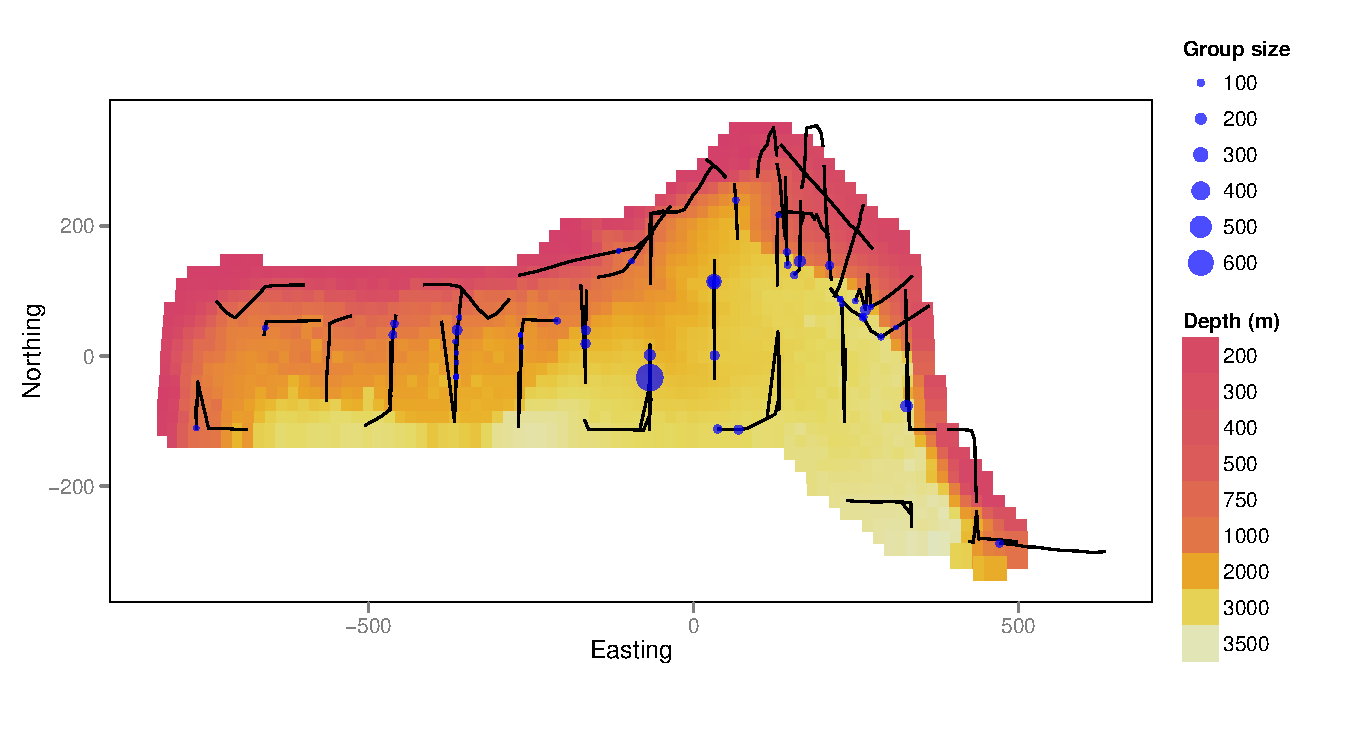
\includegraphics[width=\textwidth]{figs/depth-transects}\\
        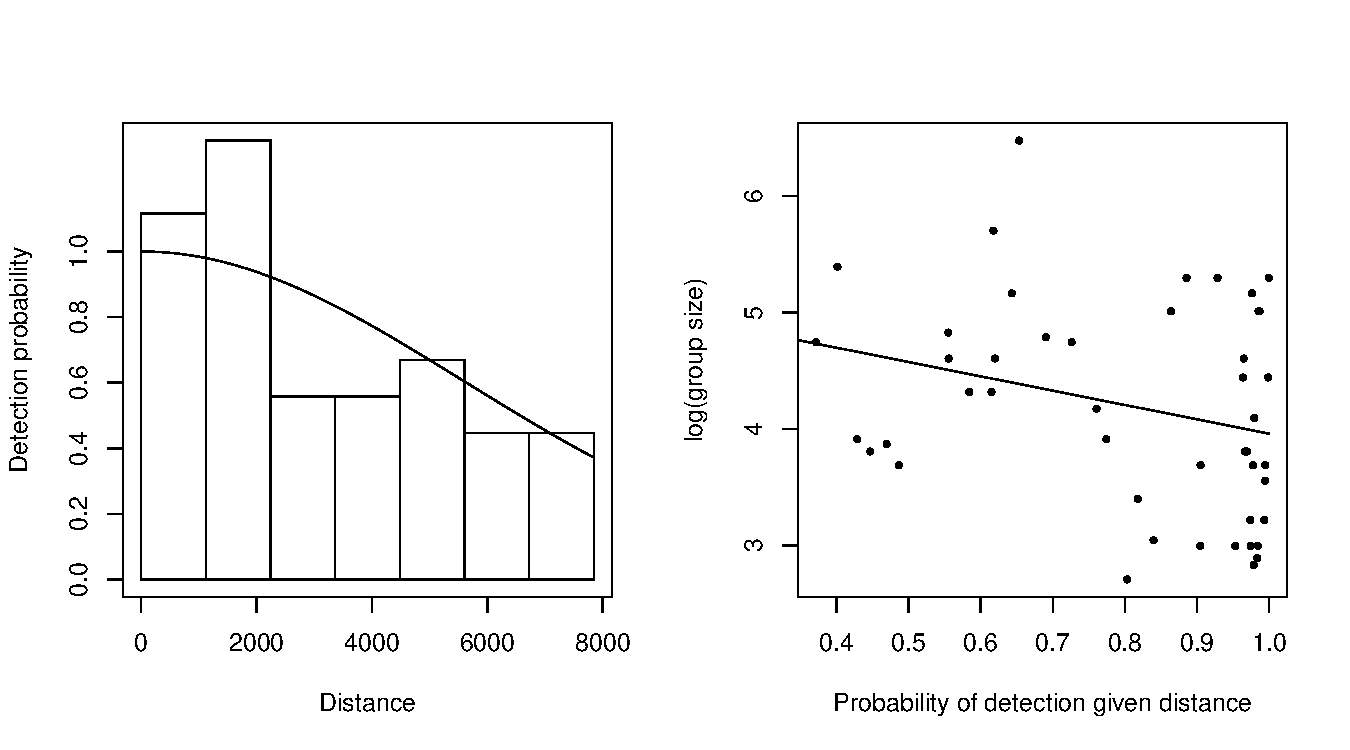
\includegraphics[width=\textwidth]{figs/distances-groups}
  \end{center}
\end{figure}

\newpage

\begin{figure}[h!]
  \caption{Predictions for the dolphin data. Top: Predictions from the model using only depth as an explanatory variable, bottom: the model using both depth and location.}
  \label{fits-depth}
  \begin{center}
    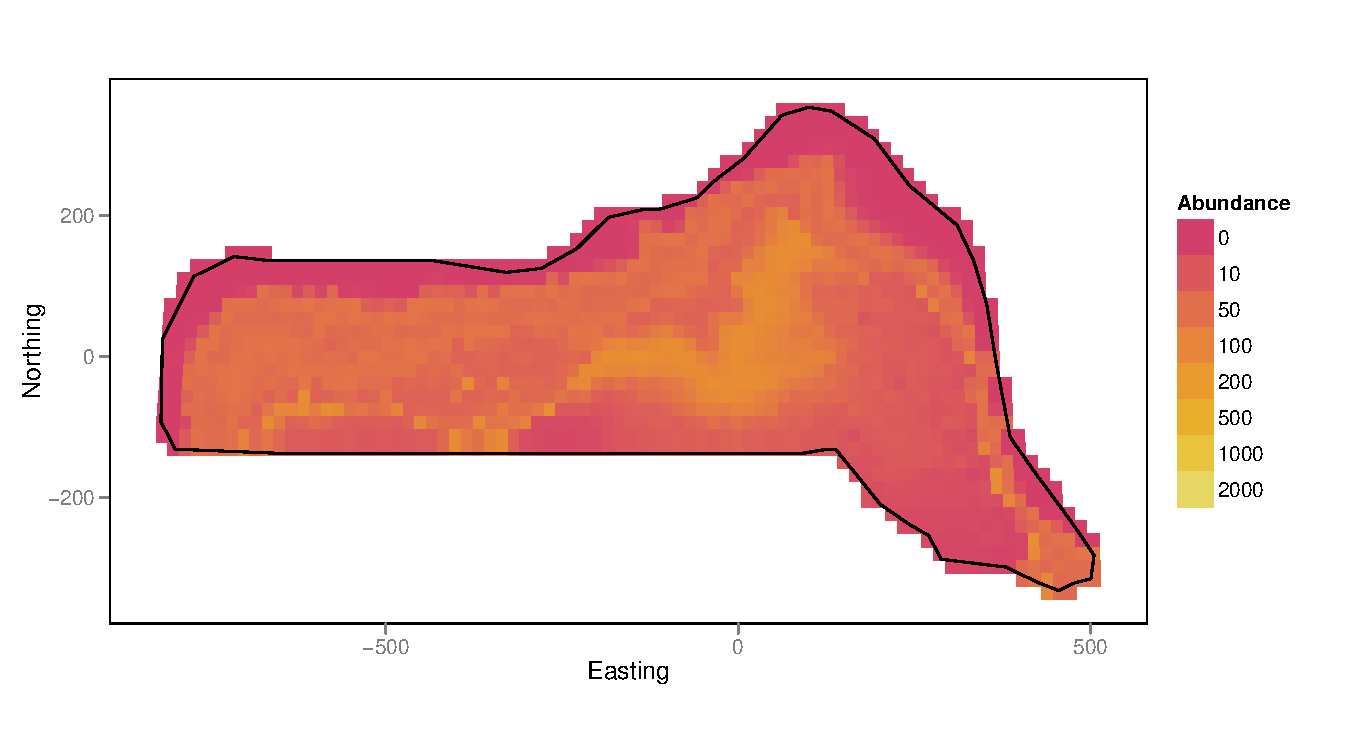
\includegraphics[width=\textwidth]{figs/fit-depth}\\
    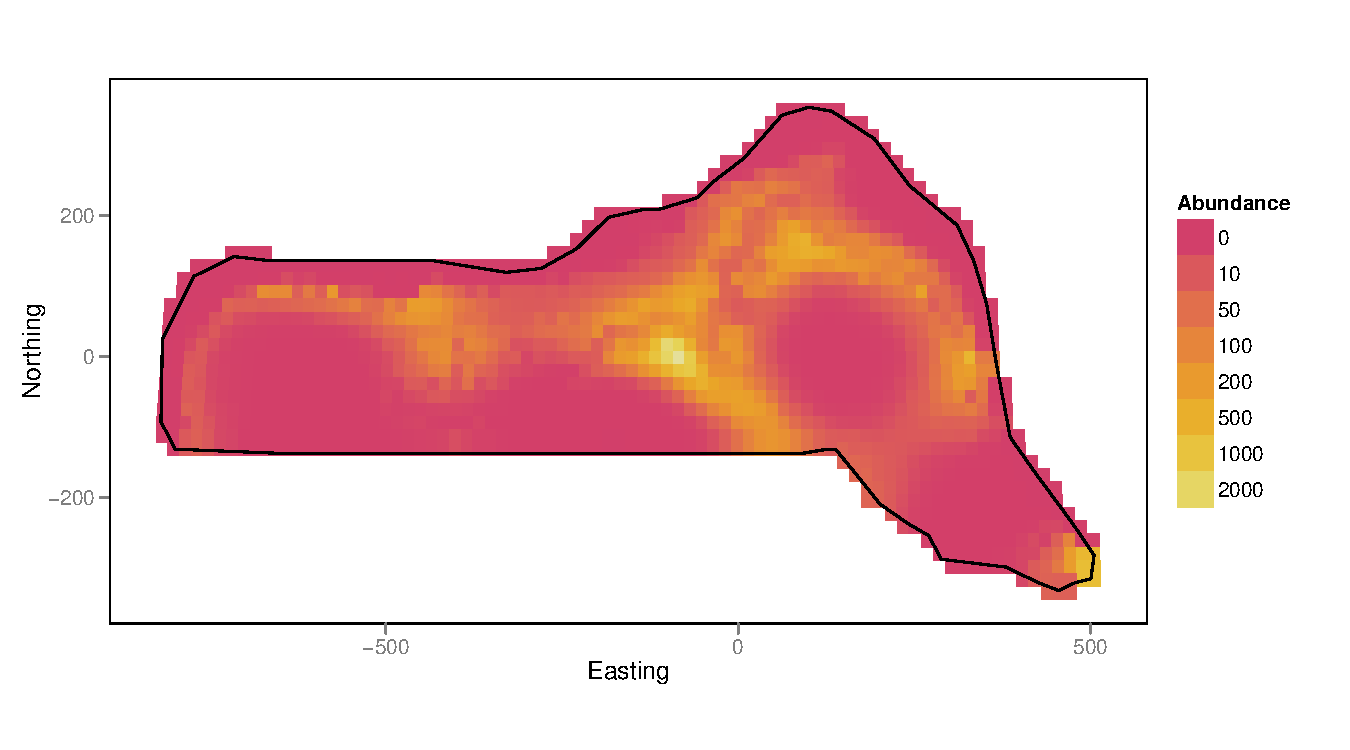
\includegraphics[width=\textwidth]{figs/fit-depth-xy}
  \end{center}
\end{figure}

\newpage

\begin{figure}[h!]
  \caption{Plot of the effect on the response of depth, note that it is possible to draw a straight line between 750m and 3000m within the confidence band, so the wiggles in the smooth may not be indicative of any relationship. What is clear is that there is some effect up to about 500m. The number in brackets on the $y$ axis indicates the effective degrees of freedom of the smooth term. The rug ticks at the bottom of the plot indicate where the data were collected.}
  \label{depth-gamplot}
  \begin{center}
    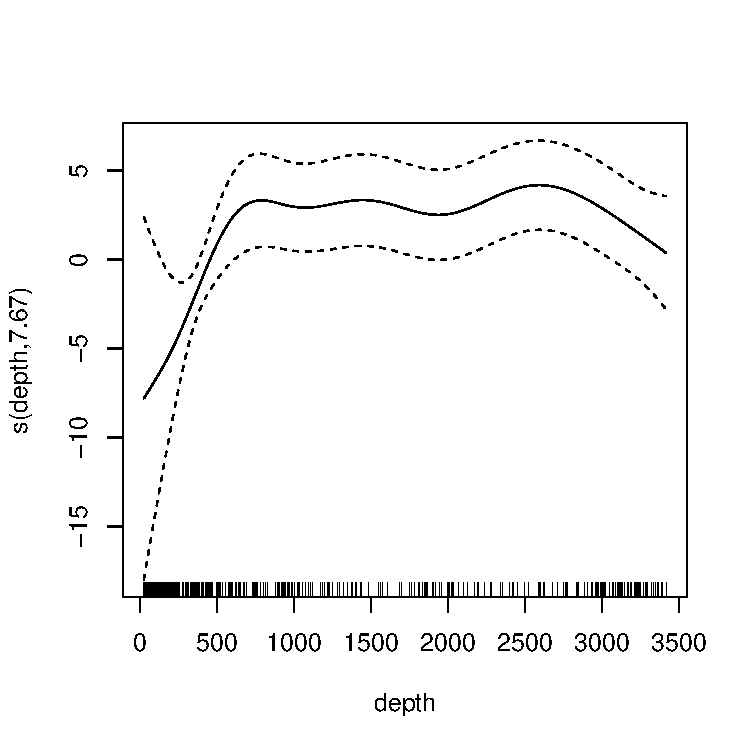
\includegraphics[width=\textwidth]{figs/fit-depth-gam}
  \end{center}
\end{figure}

\newpage

\begin{figure}[h!]
  \caption{Plot of coefficient of variation maps, showing the uncertainty in the fitted model. The top panel shows the estimate using the moving block bootstrap incorporating detection function uncertainty, the bottom panel shows the same plot using the variance propagation method. The bootstrap plot seems far more noisy.}
  \label{cv-plot}
  \begin{center}
    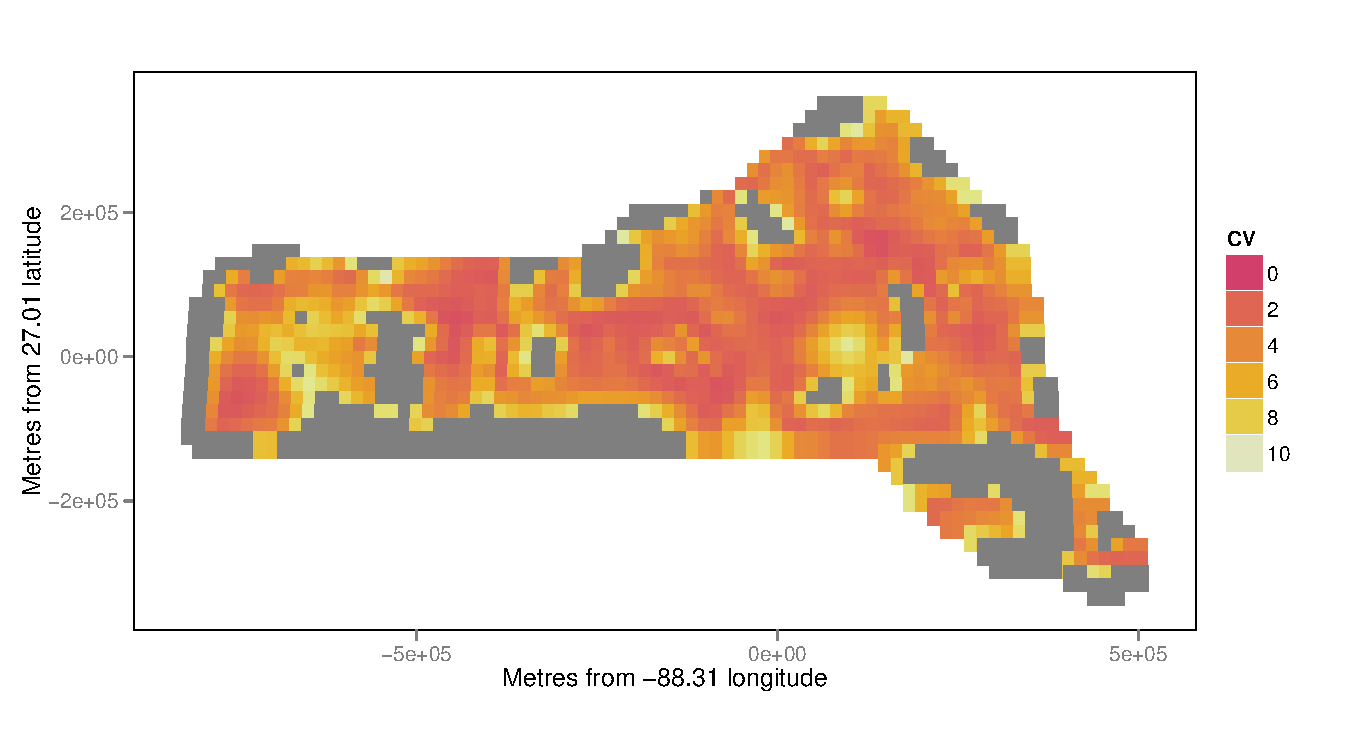
\includegraphics[width=\textwidth]{figs/cvplot-movblk}\\ 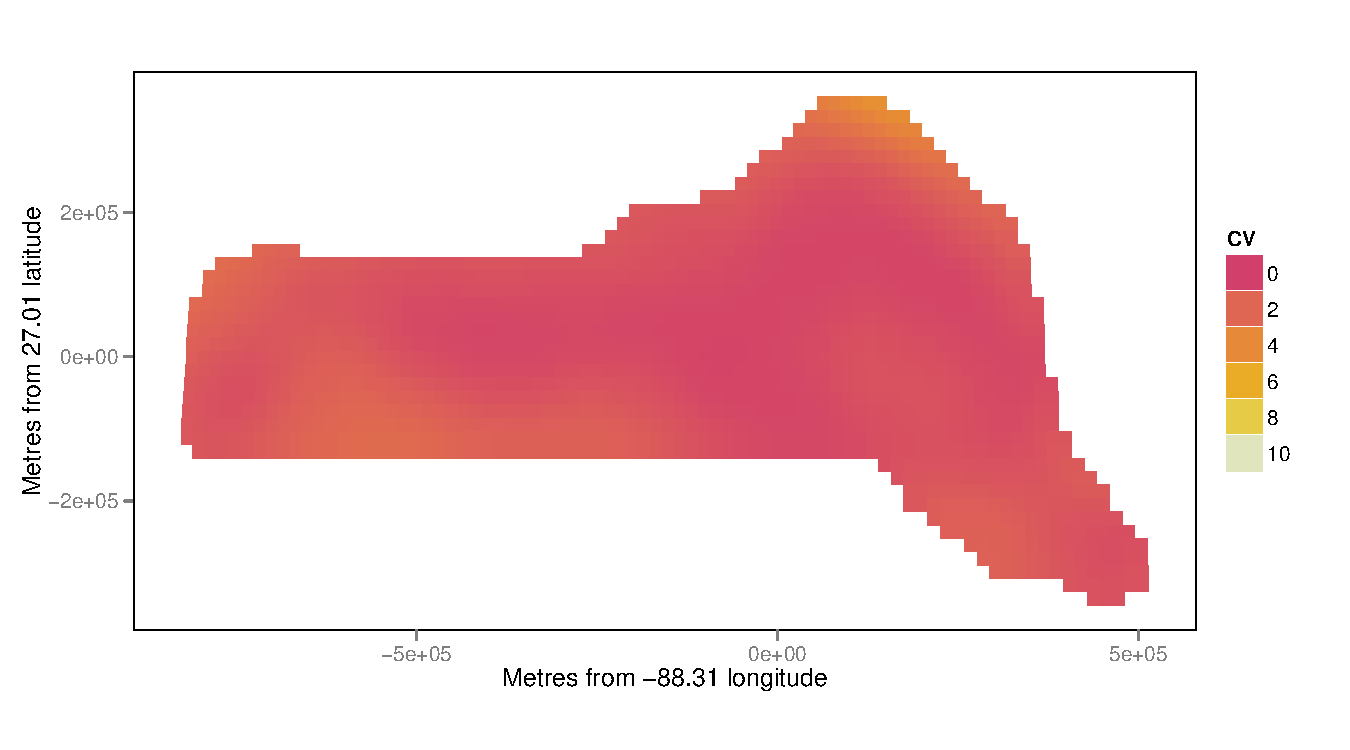
\includegraphics[width=\textwidth]{figs/cvplot-varprop}
  \end{center}
\end{figure}

\newpage

\begin{figure}[h!]
  \caption{Flow diagram showing the modelling process for creating a density surface model.}
  \label{flow}
  \begin{center}
    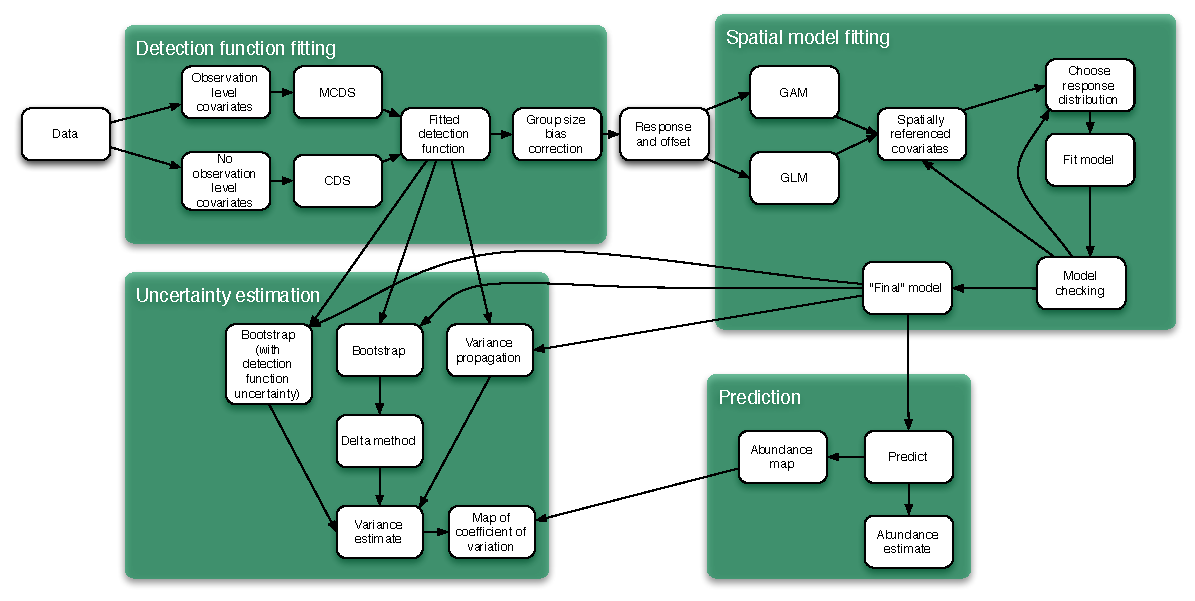
\includegraphics[width=\textwidth]{figs/flowdiagram-reduced}
  \end{center}
\end{figure}

\newpage

\begin{figure}[h!]
  \caption{Example of model diagnostics for the model which included both location and depth covariates for the dolphin data. From top left clockwise:  }
  \label{dsm-check}
  \begin{center}
    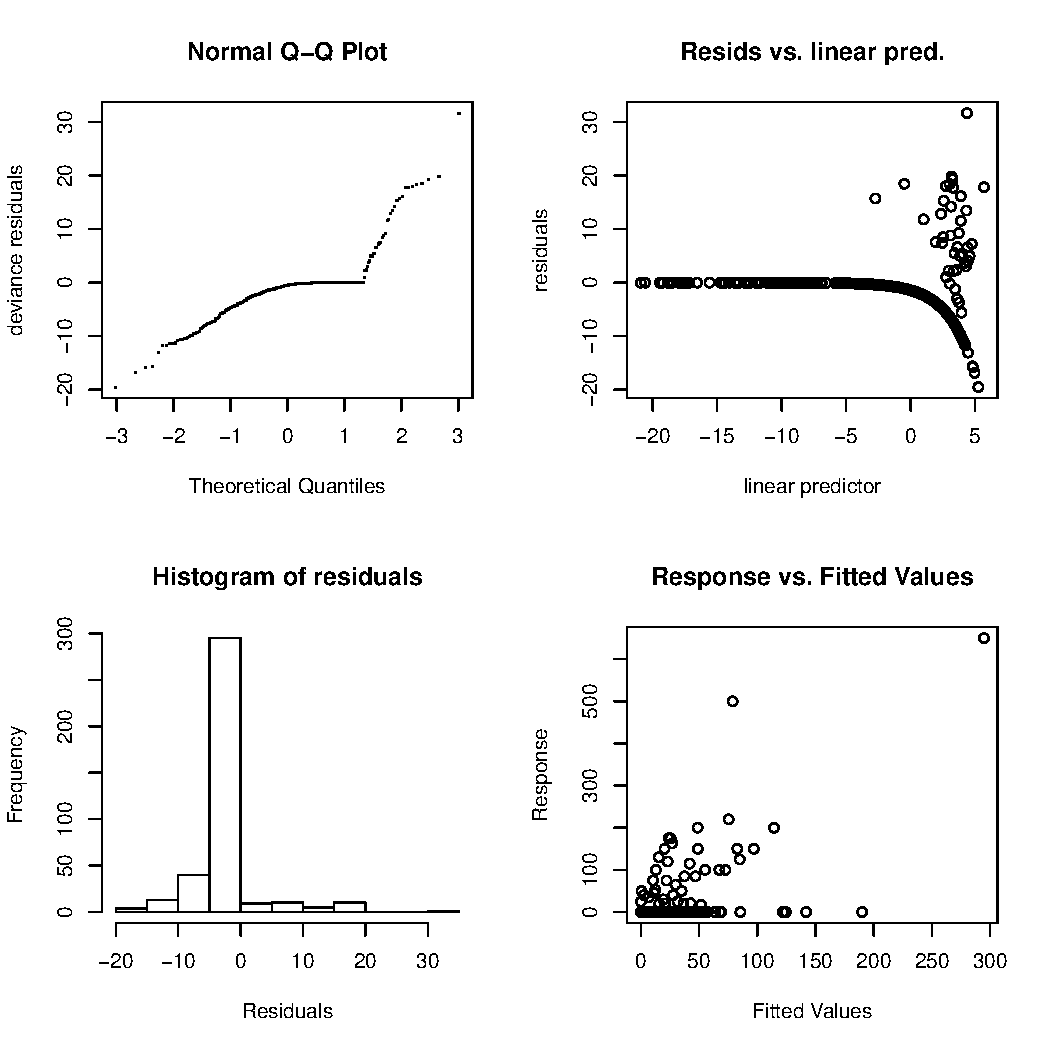
\includegraphics[width=\textwidth]{figs/dsm-check}
  \end{center}
\end{figure}


\end{document}
